\documentclass{article}
\usepackage{multicol}
\setlength{\columnsep}{1cm}
\usepackage{graphicx}
\usepackage{breqn}
\usepackage{blindtext}
\usepackage{wrapfig}
\usepackage{lipsum}
\usepackage{caption}
\usepackage{subfig}

\title{UNETs}
\author{ }
\date{March 2023}

\begin{document}
\maketitle
\begin{multicols}{2}

\section{Abstract}
U-NET is a convolutional neural network(CNN), which is used for biomedical image segmentation.
Its main advantage is the use of image augmentation, which makes training the CNN with fewer images capable. The architecture encompasses a contracting path and a symmetric expanding path.
The aim of the following project was to implement such a CNN, using the LIVECell-dataset images for training and testing the model.

\maketitle
\section{Introduction}
CNN's have been a very powerful tool in the recent years for image classification purposes.
Their advance is due the high amount of data sets that they are provided with and the dense layers (hidden layers) of neurons that its model has. 
They mimic in some ways how humans classify images,by recognizing distinct features or patterns in the image.
Furthermore the network recognizes low level features such as edges,
curves and areas of color and in the next step combines these to higher level features, for example eyes, mouth or ears, to form a better
understanding and thus makes a conclusion about the input. In the biomedical field large amount of images are difficult to be generated.
This problem is addressed with the use of image augmentation, which also strengthens the invariance of our model. The contracting path is
composed of max pooling and 3x3 convolution operations, whereas the expanding path focuses on up sampling and 3x3 convolutions. 
The paths are combined with the use of cropping and copying, with the goal being to increase localization of features, in a way that
a sequential convolution layer can create a more accurate output. The augmentation is applied with elastic image deformation.
Lastly, a weighted loss function makes the separation of cells and the background possible, with the background attaining a bigger value
of loss than the cells.
\maketitle

\section{Theory}
\subsection{Contracting Path}
As mentioned in the introduction the main tools used are convolutions and the max pooling operations. 
The convolutions use a 3x3 kernel, meaning they have 9 elements as inputs and 1 element as output. For the convolution the 
3x3 kernel is rearraged to a 4 by 16 matrix and 4x4 matrix is flattend, now with a matrix multiplication the output is a 4x1 vector, which in turn
is the convoluted matrix. \\
\begin{minipage}{5cm}
\centering
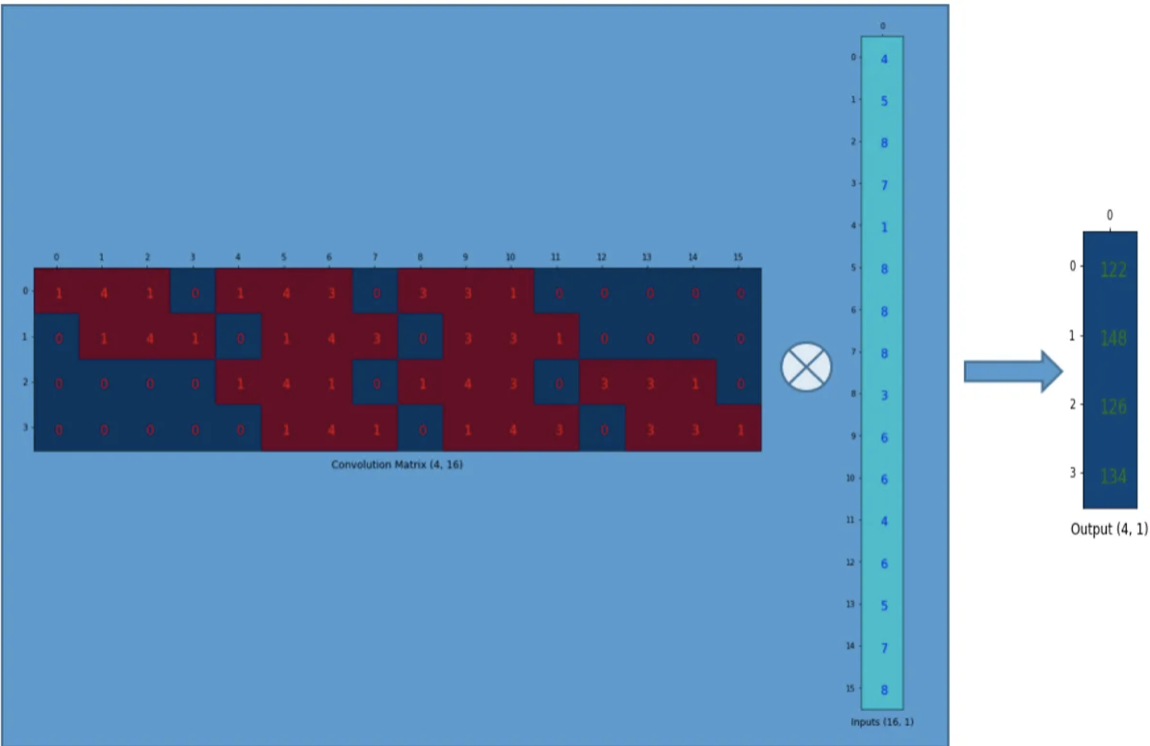
\includegraphics[width=5cm, keepaspectratio]{convolution.png}
\captionof{figure}{Covolution procedure}
\end{minipage}
\\Each element of the kernel contains a value,
which is the the weight that the corresponding element of the 4x4 matrix will be multiplied by. The higher the weight the more significant 
the element of the matrix and vice versa.
Figure 1 illustrates how convolution works. Furthermore the max pooling operation works in a similar fashion ,but instead of summing 
up the values of a n by n block it picks out the highest value of each non overlapping block reducing the matrix by a factor of n. Each layer 
has a set of features, which for the first layer they are 64 and for each consecutive layer they are multiplied by 2 until they reach 512. At the 
end of each convolution a ReLU activation function is used, which filters out all values that are smaller than 0 and gives a linear weight to 
each value above zero.  
\subsection{Expanding Path}
Since the UNET is symmetric, the expanding path mostly does the opposite procedures of the contracting path. The first operation of each layer is an up-convolution,
using a 2 by 2 kernel emulating the reverse max pooling operation followed by 3 by 3 convolutions. The upsampling path uses the transposed 
covolution matrix mutiplied with the falttend matrix of the layer, generating a larger matrix as an output. In the beginning of each upscale layer, the data
is cocatenated with the corresponding down scaled layer data after being cropped and copied. The last layer is convoluted with a 1 by 1 kernel 
in order to output the vector which contains the number of classes of each feature.

\subsection{LIVECell dataset}
The LIVECell dataset contains a wide variety of cell images and provides the user a train, test and validation split of the data via a 
.json file. Each file has a dictionary key-value structure with the main keys being the "images" and the "annotations". The "images" key has
as values the necessary information of each image, namely a designated id, name etc. and the "annotations" also have an id but in addition
hold the segmentation information and image id of each image.

\section{Implentation} 
\subsection{Preprocessing}
The dataset has two files the livecell-train-val-images and the livecell-test-images, which should be split with the help of the json files to a 
training, test and validation set. Firstly for each set, the required .json file was loaded and the names of the images of the currently used folder 
were extracted and appeded to a list. Secondly the image id and the segmentation pattern were found through the help of the names list, making 
the creation of a dictionary possible containing as key the image id and as values the segmentation pattern and the name of the image. Lastly
with the use of the polygon function, where the x coordinates are every second element starting from index one and the y coordinate being the 
same but starting from index 0, the mask of each pattern was constructed and thus the segmentation. Both the masked and original images were 
saved as grayscale in separate folders.

\subsection{Unet model}
For the implementation of the Unet the pytorch library was used. Since most operations are recurrent, a class named DoubleConv was constructed to create the main 
3x3 convolutions and the ReLU activation function, in between the BatchNorm2d was used to normalize the data with respect to the batch input and to
speed up the training process. The UNET class has as attributes the down and up path, the max pooling operation, the last 1x1 convolution and the 
bottleneck operation to create the latent space. For the up and down attributes the ModuleList is used to create the convolution procedure. Moreover 
at the end of each down iteration the MaxPool2d and on the other hand at the beginning of each up layer the ConvTranspose2d operator is used. In 
conclusion the variable skip connection is used to cocatenate the down sampled layer output with the up sampled one.   

\subsection{Dataset and \\Dataloader}
After spliting the data into the appropriate folders, the class Dataset was created in order to have access to the data and the class Dataloader was used 
in order to load the data into batches. The Dataset has besides the "init" method the "len" and "getitem" methods. The first is used to tell the dataloader the 
amount of samples that are contained in the dataset class and the second takes as input the image index to search for the specific image in the folder. Additionally, the dataloader 
optimizes the loading process by using parallel workers, which each retrieve a sample and put it into a queue until the desired batch size is reached. It is worth mentioning,
that the getitem applies some transformations to the images and the masks like augmentation and cropping, which will be discussed later.

\subsection{Loss Function and\\ Optimizer}
As an evaluation measure of the model two loss function were used, the first being weighted binary cross entropy loss(BCEL), \texttt{nn.BCEWithLogitsLoss()} from PyTorch
and not nn.BCELoss due to the "RuntimeError: Unable to find a valid cuDNN algorithm to run convolution" and the second the dice loss(DL) from the monai.losses library, which are defined as:
\begin{dmath}
BCEL= -W\sum_{n=1}^{N}y_n\cdot log(p(y_n)) +(1-y_n)\cdot log(1-p(y_n))
\end{dmath}
\begin{dmath}
DL = \frac{2*\sum_{n=1}^{N}p_ig_i}{\sum_{n=1}^{N}p_i^2 + \sum_{n=1}^{N}g_i^2}
\end{dmath}
Entropy is a measure for uncertainty of a given distribution and the weighted BCEL calculates the probability that a specific pixel is either a boundary pixel or a background pixel and
adds some weight to it in the training process, for example a boundary pixel would have a much larger weight than a background pixel. After finding each pixels probability the mean is computed to find the resulting loss. 
The problem of this method is that the per-pixel loss is determined in a way without knowing if the neighbouring pixels are boudary pixels or not. 
This is the advantage of the dice loss function, with $p_i$ and $g_i$ representing whether a pixel is a boundary pixel(1) or not(0). The denominator 
being the sum of total boundary pixels and the numerator is the sum of correctly predicted boundary pixels because the sum increments only when $p_i$ and $g_i$ match.
The optimizer used is the Adams optimzer, with the configuration parameters being the learning rate, exponential decay and lastly the AMSGrad to solve the possible
convergence problem of the Adam algorithm.

\subsection{Augmentation and Cropping}
To increase the invariance of the model and variability of images, they were augmented in the dataset class, via the use of the function \texttt{elastic_transform()},
which is a elastic deformation of the image. The deformation is applied via the use of the \texttt{GaussianBlur()} function from the cv2 library and the main parameters are 
sigma for the variance and alpha is the scaling factor that controls the intensity of the deformation in the y and x directions. In addation to the first transformation a 
rotation was also applied. The images were first only resized, but this resulted in a loss of quality and thus a blurry image, as Figure 2 illustrates. 
\noindent
\begin{minipage}{\columnwidth}
  \makeatletter
  \newcommand{\@captype}{figure}
  \makeatother
  \centering
  \subfloat[Resized image]{%
    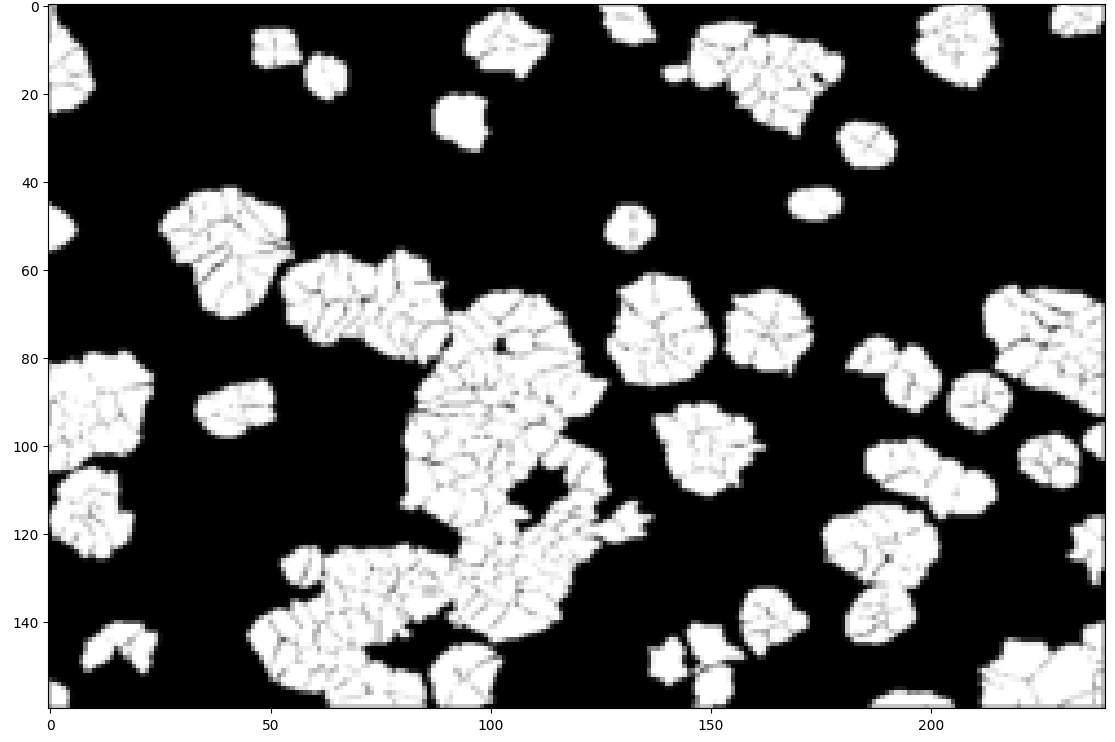
\includegraphics[width=5cm]{lossofquality1.png}%
    \label{fig:evaluation:revenue}%
  }\qquad%
  \subfloat[Prediction of resized image]{%
    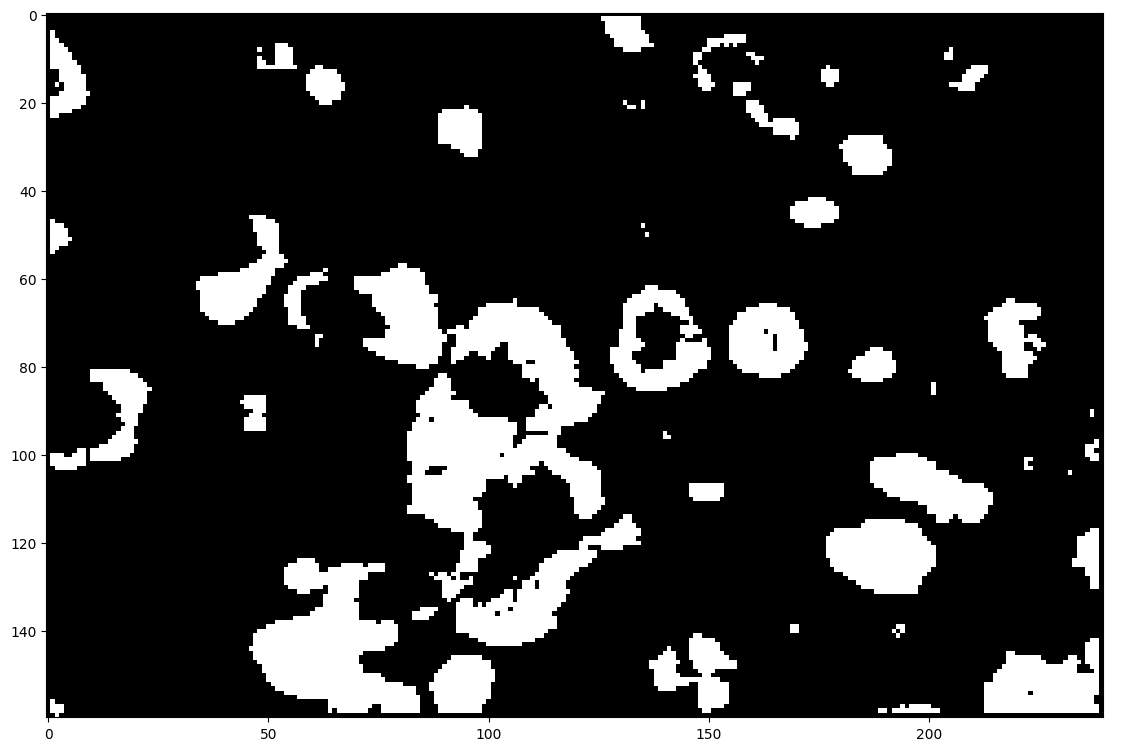
\includegraphics[width=5cm]{lossofquality0-2.png}%
    \label{fig:evaluation:avgPrice}%
  }
  \caption{Resizing without cropping}
\end{minipage}
To fix this issue the batch size was minimized to 2 ,then the images and masks were cropped with the purpose of having the same aspect ration, which is \texttt{image_height=333}
and \texttt{image_width=434}, which resulted in not needing a resize.

\subsection{Training, Validation \\and Testing}
The training process was split into two parts, the first part was using only the normal images without applying any transformations and the second was using all 
the transformations mentioned above, resulting into a double sized training set. The augmentation was done inside the training set to  ensure that each batch of training data is different from the previous one
which can help prevent overfitting and improve the generalization performance of the model. The validation and test dataset did not get augmented, instead only cropped.

\section{Results}

\end{multicols}
\end{document}
% \begin{figure*}[p]
% \begin{minipage}{5cm}
% \centering
% 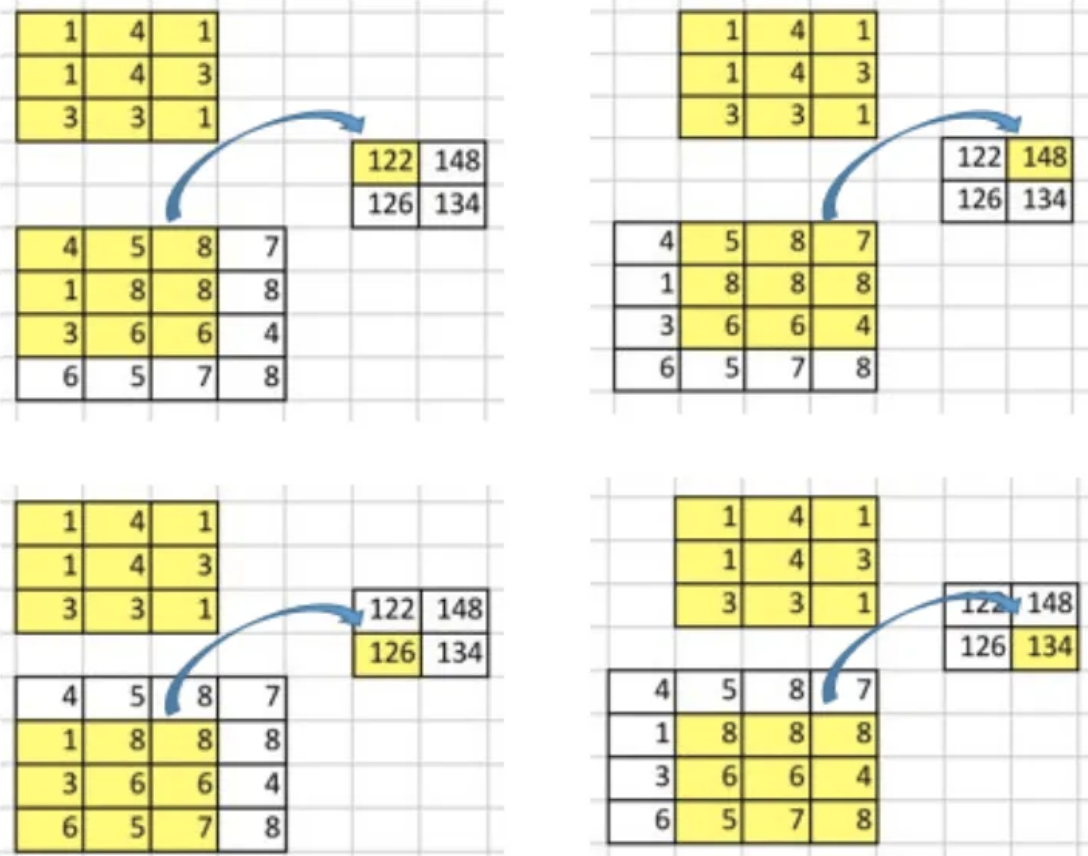
\includegraphics[width=5cm, keepaspectratio]{downsampling.png}
% \captionof{figure}{Downsampling}
% \end{minipage}

% \end{figure*}